\documentclass[12]{article}
\usepackage[utf8]{inputenc}
\usepackage{cite}
\author{par4111 \\ Adrià Cabeza, Xavier Lacasa \\ Departament d' Arquitectura de Computadors}
\title{Lab 1: Experimental setup and tools}
\date{\today \\ 2018 - 19 PRIMAVERA}
\usepackage{graphicx}
\usepackage{subcaption}

\begin{document}
\maketitle
\newpage
\tableofcontents
\newpage
\section{Introduction}
In order to do properly this subject, first, we have to introduce some new concepts and hardware and software environment that we will use during this semester to do all laboratory assignments.  The following document contains an introductory approach, step by step introducing those concepts. We will introduce the \textit{Boada} architecture, some of the most important parallelism concepts and several tests to see its effects. 

\section{Experimental setup}
\subsection{Node architecture and memory}

\textit{Boada} is a multiprocessor server located at the Computer Architecture Department divided in different nodes, each of them with different architecture and diffferent uses. \textit{Boada} is composed of 8 nodes (from boada-1 to boada-8) and they can be grouped as the following table: 
\\
\begin{table}[h]
\begin{tabular}{|l|l|l|l|}
\hline
Node name    & Processor generation                & Interactive & Queue name \\ \hline
boada-1      & Intel Xeon E5645                    & Yes         & batch      \\
boada-2 to 4 & Intel Xeon E5645                    & No          & execution  \\
boada-5      & Intel Xeon E5-2620 v2 + Nvidia K40c & No          & cuida      \\
boada-6 to 8 & Intel Xeon E5-2609 v4               & No          & execution2 \\ \hline
\end{tabular}
\end{table}

However in this course we are going to use mainly from boada-1 to boada-4. The easiest way to obtain the information of the hardware used in each node is using the linux commands lscpu and lstopo(~\ref{fig:lstopto2} and ~\ref{fig:lstopto8}). This commands can be easily executed in the boada-1 node (because it is interactive), but if we want to use the other nodes we can use the submit-*.sh script provided by the PAR teachers and use the queue system. \\
\medskip

\begin{figure}[h]
  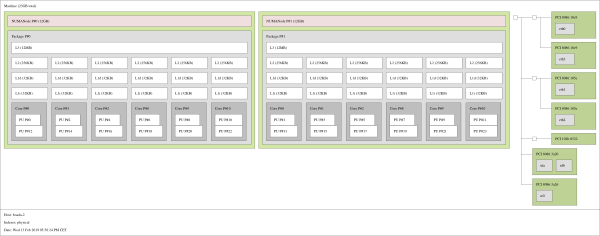
\includegraphics[width=.8\linewidth]{map-2.png}
  \caption{Boada-2 architecture outputed by lstopo. }
  \label{fig:lstopto2}
\end{figure}

\begin{figure}[h]
  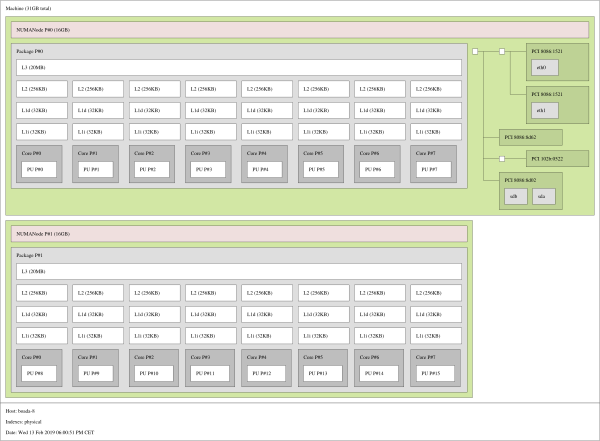
\includegraphics[width=.8\linewidth]{map-8.png}
  \caption{Boada-8 architecture outputed by lstopo. }
  \label{fig:lstopto8}
\end{figure}

After creating the scipts and applying them to each of the nodes, we obtained the following hardware information: 


\begin{table}[h]
    \begin{tabular}{|l||l|l|l|}
    \hline
                                        & boada-1 to boada-4    & boada-5   & boada-6 to boada-8    \\
    \hline\hline
    Number of sockets per node          & 2                     & 2         & 2                     \\
    \hline
    Number of cores per socket          & 6                     & 6         & 8                     \\
    \hline
    Number of threads per core          & 2                     & 2         & 1                     \\
    \hline
    L1-I cache size (per-core)          & 32 KB                 & 32 KB     & 32 KB                 \\    
    \hline
    L1-D cache size (per core)          & 32 KB                 & 32 KB     & 32 KB                 \\
    \hline
    L2 cache size (per-core)            & 256 KB                & 256 KB    & 256 KB                \\
    \hline
    Last-level cache size (per-socket)  & 12 MB                 & 15 MB     & 20 MB                 \\
    \hline
    Main memory  size (per socket)      & 12 GB                 & 31 GB     & 16 GB                 \\
    \hline
    Main memory size (per node)         & 23 GB                 & 63 GB     & 31 GB                 \\
    \hline
    \end{tabular}
\end{table}

\bigskip

The previous table gives us really powerful information that will be necessary in the future to properly use the \textit{boada} system and understand the parallelism decomposition and time we will get. 

\subsection{Sequential and parallel executions}

\subsubsection{Strong scalability}
\subsubsection{Weak scalability}

\section{Experimental setup}
\subsection{Introduction}
The objective of this laboratory is learn how to use Tareador, an environment to analyse the potential parallelilsm that can be obtained when a certain task decomposition is applied to a code. We will introduce how it works and we will experiment and analyse decomposition with a sequential code called 3DFFT.

\subsection{Analysis of task decompositions for 3DFFT}
\begin{table}[h]
\begin{tabular}{|l|l|l|l|}
\hline
Version & $T_1 $ & $T_\infty$ & Parallelism \\ \hline
seq     &   &   &             \\ \hline
v1      &   &   &             \\ \hline
v2      &   &   &             \\ \hline
v3      &   &   &             \\ \hline
v4      &   &   &             \\ \hline
v5      &   &   &             \\ \hline
\end{tabular}
\end{table}

\section{Conclusions}

\end{document}
